\chapter{Manipulator Kinematics}  
\label{chap:manip}

 
Recommended Text Readings: 
\begin{itemize}
 \item \cite[Chapter 3]{MurrayBook}
 %
 \item \cite{Brockett1990}
 %
 \item \cite[Chapter 4]{LynchBook}
\end{itemize}

At issue in this chapter is characterizing the \textit{motion} of a robot based on the position and orientation of the links of the robot (in the case of rigid bodies). We will leave discussion of the forward or differential kinematics of soft robots to a future discussion but we will briefly discuss it in class. First off, based on the first chapter of ~\cite{Hunt1983}'s Kinematic Geometry of Mechanisms, we recollect that there are six primitive types of joints constructed from the so-called \textit{lower pairs} of mechanisms, which all exercise a subgroup of \textit{SE(3)} when they are actuated.


\section{Forward kinematics}
%
Formally, we define the \textit{forward kinematics of a robot as a means of finding the configuration of the end-effector when we are given only the relative configurations of each pair of adjacent links of the robot}. For an open-loop kinematic chain, these adjacent links are the joint angles while for a parallel robot, they are the link lengths of the robot's legs. A similar definition applies to a semi-rigid multi-dof soft robot, whereupon we are tasked with finding the orientation of the tool frame given a characterization of the \textit{deformation} of the adjoining soft or semi-rigid links of the soft robot's body. 
%
\begin{figure}[tb!]
	\centering
	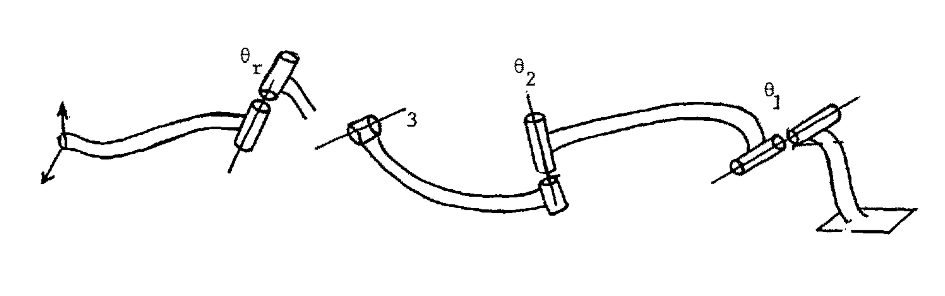
\includegraphics[width=.8\columnwidth]{figures/manip.png}
	\caption{An open kinematic chain. Reprinted from \cite{Brockett1990}.}
	\label{fig:manip}
\end{figure}
%
\begin{figure}[tb!]
	\centering
	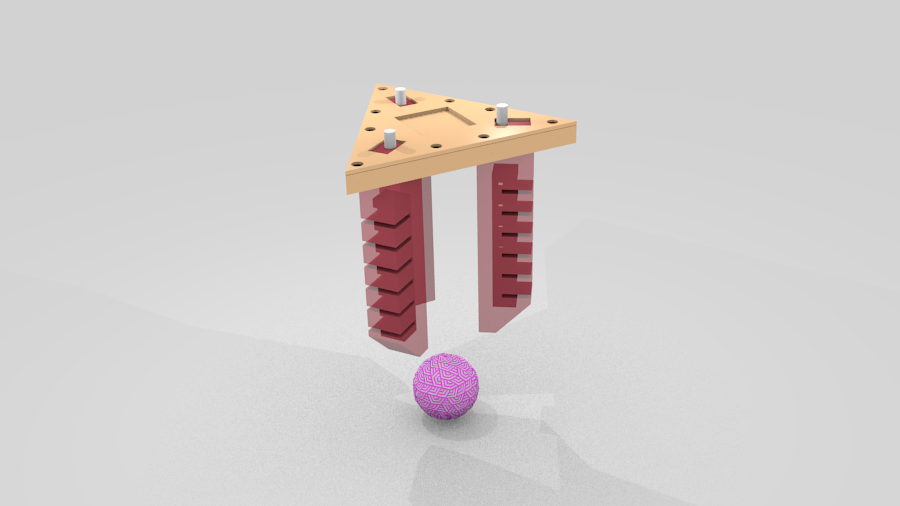
\includegraphics[width=.8\columnwidth]{figures/pneunets.png}
	\caption{The Pneunets Soft Robot}
	\label{fig:pneunets}
\end{figure}
%

\subsection{Screw Axes and  Base Frame}

For consider the kinematic chain of \autoref{fig:manip}. Suppose that we fix a right-handed triad of orthogonal vectors at the tip of each member of the chain, the\textit{ joint space} $Q$ of the robot is the set of all possible values of the joint variables of the robot, which happens to also be the C-space of the robot given that the joint angles completely determine the locations of every link in the robot. 
Similarly, for the soft robot of \autoref{fig:pneunets}, we construct the forward kinematics in a similar fashion; only this time, we do not parameterize the robot links with the joint angles but with the appropriate representation of the deformation of the each pneunet link: an example of a common parameterization approach is to use differential kinematics for arc on the soft robot's body~\cite{Hannan2003}.
%%

For the arm of \autoref{fig:manip}, we may consider that every joint applies a screw motion to all links that protrude from the robot. We take each joint to be displaced by some angle $\theta_i$ so that the end-effector undergoes a displacement of the form $e^{\hat{\xi}_i \theta_i}\homo_i$. The cumulative effect of the robot links on the end-effector is given as (following the notation of \autoref{fig:lienotations}),
%
\begin{align}
\homo_{st}(\theta_1, \ldots, \theta_l) = e^{\hat{\xi}_1 \theta_1}\,e^{\hat{\xi}_2 \theta_2}  \, \ldots e^{\hat{\xi}_l \theta_l} \homo_{st}(0)
\label{eq:fwd_kine}
\end{align}
%
\textit{where $S$ denotes the spatial frame, typically located at the base or shoulder of the robot and $T$ denotes the tool frame, typically situated at the robot's end-effector}. For the system of \eqref{eq:fwd_kine}, we say $\xi_i$ is the twist coordinate of the $i'th$ joint. The equation is the result of moving $\theta_{i+1}$ first before $\theta_i$ while keeping $\theta_i$ fixed. On the other hand, if we reverse the order of the rotations, that would correspond to moving the $i'th$ axis and then rotating the $(i+1)'th$ axis about the new axis, \ie,
%
\begin{align}
	\xi_{i+1}^\prime = \text{Ad}_{e^{\hat{\xi}_i \theta_i}} \xi_{i+1}.
\end{align}
%
We note that the the twist for a revolute joint takes the following form
%
\begin{align}
	\xi_i = \left(\begin{array}{c}
	-\omega \times q_i \\ q_i
	\end{array}\right)
\end{align}
%
where $\omega_i \in \bb{R}3$, is the unit vector in the direction of the twist axis and $q_i \in \bb{R}^3$ is a point along that axis. For a prismatic joint, we have $\xi_i = (v_i, 0)^T$ where $v_i$ is a unit vector along the direction of translation.

\begin{figure}
	\centering
	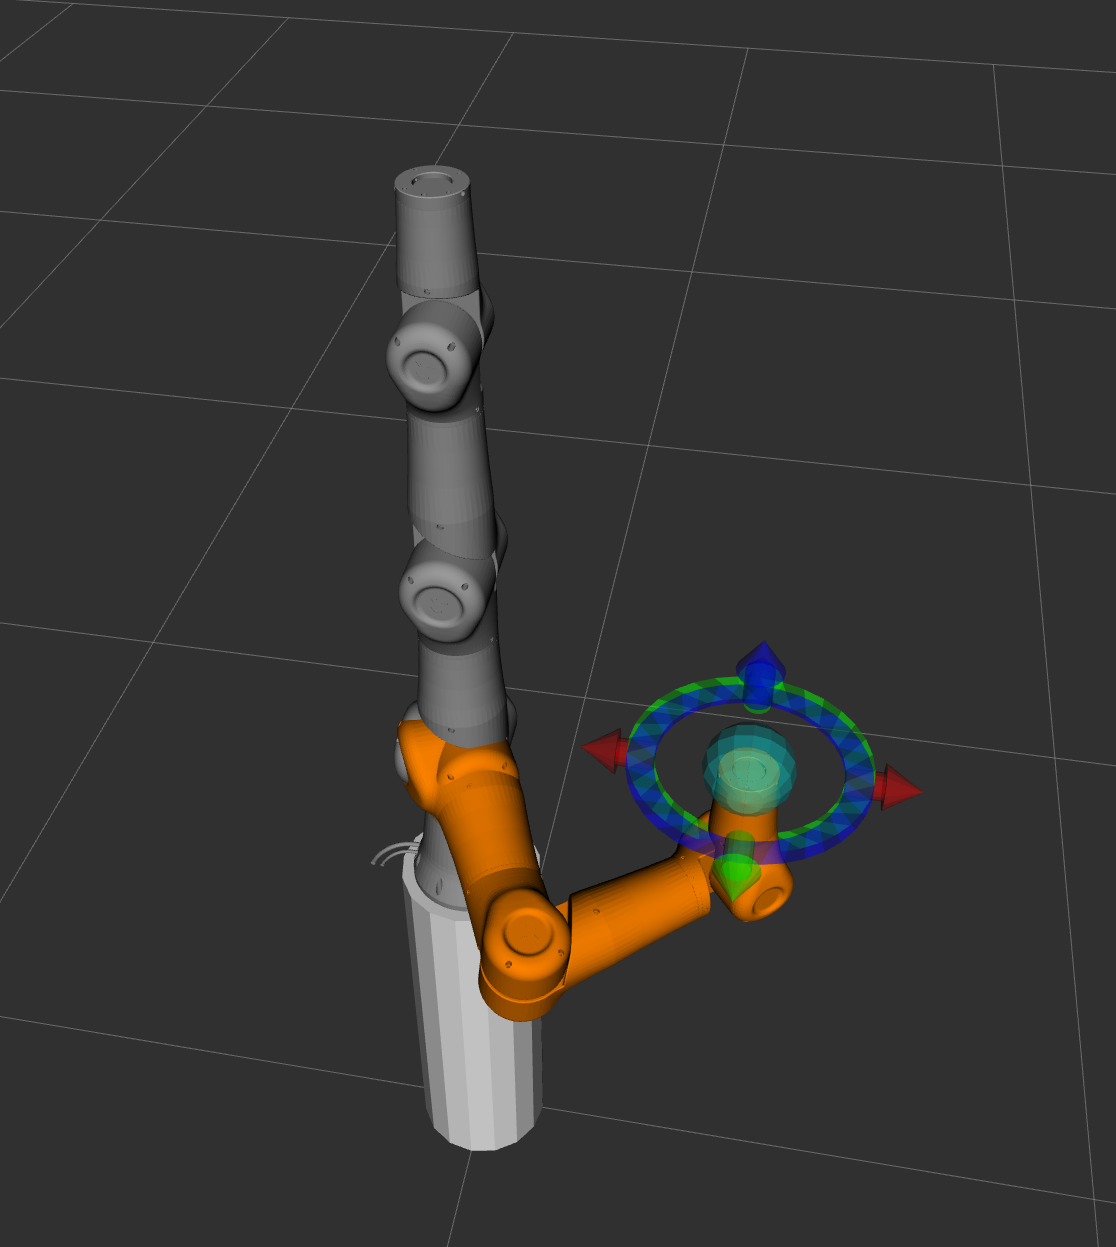
\includegraphics[width=\columnwidth]{figures/torobo7.png}
	\caption{Forward Kinematic Planning for The Torobo 7 Arm}
	\label{fig:torobo7}
\end{figure}
%
\begin{example}
	Consider the Tokyo Robotics (Torobo) arm of \autoref{fig:torobo7}, which is made up of seven joints (six actually, but for now we will assume there is a planar wrist at the end-effector for grasping). The Cartesian coordinates triad are as shown in the orange-colored configuration wherin the blue axis is z, the red axis is $y$-axis and the green axis denotes the $x$-axis. We will take the home position of the robot to be when all joint angles have their angles as $\theta_i = 0$ (this corresponds to the gray pose in the figure). The target pose of the arm is the orange-linked arm shown. The forward kinematics problem would be that given all the six joint angles, and link lengths, find the end-effector pose. We will be leveraging Brockett's product of exponential formula in solving this problem.
	
	For now, suppose the spatial frame is at the base of the robot and the tool frame is on the end-effector. We will for the moment assume that the end-effector is posed at an angle $\theta_7= 0$ as well in the reference frame (colored in gray). The transformation from the base frame to the tool frame is at $\theta = 0$ so that we have from \eqref{eq:fwd_kine}
	%
	\begin{subequations}
		\begin{align}
		&g_{st}(\theta_1,\theta_2,\theta_3,\theta_4,\theta_4, \theta_5, \theta_6, \theta_7) =	e^{\hat{\xi}_1 0}\,e^{\hat{\xi}_2 0},  \, \ldots, e^{\hat{\xi}_l 0} \homo_{st}(0)   \\
		%
		g_{st}(\bm{\theta}) & = g_{st}(0) = \left(\begin{array}{cc}
		\rot(\theta=0) & d \\
		0 & 1
		\end{array} 
		\right) = \left(
		\begin{array}{cc}
		\identity & \left(\begin{array}{c}
		0 
		\\
		%
		0
		\\
		%
		\sum_{i=1}^{i=6} l_i
		\end{array}\right)  \\
		0 & 1
		\end{array} \right).
		\end{align}
	\end{subequations}
\label{ex:torobo7}
\end{example}

\subsection{Screw Axes in Tool Frame}
%
Now, consider again \eqref{eq:fwd_kine}, and recall the properties of the exponential map as given in Def. \autoref{def:exp_map}, we can write 
%
\begin{subequations}
	\begin{align}
	e^{\homo^{-1}P\homo} &= \homo^{-1} e^{P} \homo \\
	\homo \, e^{\homo^{-1}P\homo} &= \homo \, \homo^{-1} e^{P} \homo = e^{P} \homo 
	\end{align}
	\label{eq:mat_exp_reorder}
\end{subequations}
%
Reordering \eqref{eq:fwd_kine} by repeatedly applying \eqref{eq:mat_exp_reorder}, we find that
%
\begin{subequations}
	\begin{align}
	\homo_{st}(\theta_1, \ldots, \theta_l) &= e^{\hat{\xi}_1 \theta_1}\,e^{\hat{\xi}_2 \theta_2}  \, \ldots e^{\hat{\xi}_l \theta_l} \homo_{st}(0) \\
	%
	&= e^{\hat{\xi}_1 \theta_1}\,e^{\hat{\xi}_2 \theta_2}  \, \ldots \homo e^{\homo^{-1} \twistmap_l \homo \theta_l}  \\
	%
	&= e^{\hat{\xi}_1 \theta_1}\,e^{\hat{\xi}_2 \theta_2}  \, \ldots \homo e^{\homo^{-1} \twistmap_{l-1}\homo\theta_{l-1}} e^{\homo^{-1} \twistmap_{l} \homo \theta_l}  \\
	%
	&= e^{\hat{\xi}_1 \theta_1}\,\homo e^{\homo^{-1} \twistmap_{2}\homo\theta_{2}}   \, \ldots e^{\homo^{-1} \twistmap_{l-1}\homo\theta_{l-1}} e^{\homo^{-1} \twistmap_{l} \homo \theta_l}   \\
	%
	&= \homo e^{\homo^{-1} \twistmap_{1}\homo\theta_{1}}  \, e^{\homo^{-1} \twistmap_{2}\homo\theta_{2}}   \, \ldots e^{\homo^{-1} \twistmap_{l-1}\homo\theta_{l-1}} e^{\homo^{-1} \twistmap_{l} \homo \theta_l}  
	\end{align}
	\label{eq:fwd_kine_rev}	
\end{subequations}
%
or 
%
\begin{tcolorbox}[title=Exponential Map in Tool Frame]
	\begin{align}
		\homo_{st}(\theta_1, \ldots, \theta_l) &= \homo e^{\hat{\bodyform}_1\theta_{1}}  \, e^{\hat{\bodyform}_2 \theta_{2}}   \, \ldots e^{\hat{\bodyform}_{l-1} \theta_{l-1}} e^{\hat{\bodyform}_{l} \theta_l} 
	\end{align}
	where $\hat{\bodyform}_i = \homo^{-i} \twistmap_{i}\homo^{i}$ is referred to as the \textbf{body form} of the POE formula. The expression in \eqref{eq:fwd_kine} is notably called the \textbf{space form} of the POE formula.
\end{tcolorbox}

\section{Manipulator parameterization with twists}
%
In the example of \autoref{ex:torobo7}, we can construct the twists for the revolute joints as 
%
\begin{align}
	\omega_1 = \omega_2 = \ldots = \omega_7 = \left(\begin{array}{c}
	0 \\ 0 \\ 1
	\end{array}\right)
\end{align}
%
so that we can choose axis points 
%
\begin{align}
	q_1 &= \left(\begin{array}{c}
	0 \\ 0 \\ l_0
	\end{array}\right) \, 
	%
	q_2 = \left(\begin{array}{c}
	0 \\ 0 \\ l_1
	\end{array}\right) \, 
	%
	q_3 = \left(\begin{array}{c}
	0 \\ 0 \\ l_1 + l_2
	\end{array}\right) \, 
	%
	q_4 = \left(\begin{array}{c}
	0 \\ 0 \\ l_1 + l_2 + l_3
	\end{array}\right) \, 
	%
%	q_4 = \left(\begin{array}{c}
%	0 \\ 0 \\ \sum_{i=1}^{i=4} l_i
%	\end{array}\right) 
	\\
	%	
	q_5 &= \left(\begin{array}{c}
	0 \\ 0 \\  \sum_{i=1}^{i=4} l_i
	\end{array}\right) \, 
	%
	q_6 = \left(\begin{array}{c}
	0 \\ 0 \\  \sum_{i=1}^{i=5} l_i
	\end{array}\right) \, 
	%
	q_7 = \left(\begin{array}{c}
	0 \\ 0 \\  \sum_{i=1}^{i=6} l_i
	\end{array}\right).
\end{align}
%
It follows that we may write the twist as 
%
\begin{subequations}
	\begin{align}
	\xi_1 &= \left(\begin{array}{c}
	0 \\ 0 \\ 0 \\ 0\\ 0 \\ 0 
	\end{array}\right) \, 
	%
	\xi_2 = \left(\begin{array}{c}
	0 \\ 0 \\ 0 \\ 0\\ 0 \\ l_1
	\end{array}\right) \, 
	%
	\xi_3 = \left(\begin{array}{c}
	0 \\ 0 \\ 0 \\ 0 \\ 0 \\ l_1 + l_2
	\end{array}\right) \, 
	%
	\xi_4 = \left(\begin{array}{c}
	0 \\ 0 \\0 \\ 0 \\  l_1 + l_2 + l_3
	\end{array}\right) \, \\
	%\end{align}
	%%
	%\begin{align}
	\xi_5 &= \left(\begin{array}{c}
	0 \\ 0 \\ 0 \\ 0 \\ 0 \\ \sum_{i=1}^{i=4} l_i
	\end{array}\right) \, 
	%
	\xi_6 = \left(\begin{array}{c}
	0 \\ 0 \\  0 \\ 0 \\ 0 \\ \sum_{i=1}^{i=5} l_i
	\end{array}\right) \, 
	%
	\xi_7 = \left(\begin{array}{c}
	0 \\ 0 \\   0 \\ 0 \\ 0 \\ \sum_{i=1}^{i=6} l_i
	\end{array}\right)
	\end{align}
\end{subequations}
%
where the screw axes in the base frame are as given in \autoref{tab:torobo_screw_space_form}
%
\begin{table}[tbph!]
	\caption{Table of Screw Axes for the Torobo Arm.}
	\centering
	\begin{tabular}{|c|c|c|| c|c|c|}
		\hline \rule[-2ex]{0pt}{5.5ex}  
		$i$ & $\omega_i$ & $v_i$ & $i$ & $\omega_i$ & $v_i$\\
		\hline \rule[-2ex]{0pt}{5.5ex}  
		1  & (0, 0, 0) & (0, 0, 0) & 4  & (0, 0, $l_1+l_2+l_3$) & (0, 0, 0) \\	
		\hline \rule[-2ex]{0pt}{5.5ex}  
		2  & (0, 0, $l_1$) & (0, 0, 0) & 5  & (0, 0, $l_1+l_2+l_3+l_4$) & (0, 0, 0)  \\
		\hline \rule[-2ex]{0pt}{5.5ex}  
		3  & (0, 0, $l_1+l_2$) & (0, 0, 0) & 6  & (0, 0, $l_1+l_2+l_3+l_4+l_5$) & (0, 0, 0)  \\
		\hline \rule[-2ex]{0pt}{5.5ex}  
		7  & (0, 0, $l_1+l_2+l_3+l_4+l_5+l_6$) & (0, 0, 0)  & 7  & (0, 0, $l_1+l_2+l_3+l_4+l_5+l_6$) & (0, 0, 0) \\
		\hline
	\end{tabular}
\label{tab:torobo_screw_space_form}
\end{table}
%
We may now write the various exponents as 
%
\begin{subequations}
	\begin{align} 
	e^{\hat{\xi}_1 \theta_1} &= \left(\begin{array}{cccc}
	\cos \theta_1 & -\sin \theta_1 & 0 & 0 \\
	\sin \theta_1 & \cos \theta_1 & 0 & 0 \\
	0 & 0 & 1 & 0 \\
	0 & 0 & 0 & 1
	\end{array}\right), \quad
	%	
	e^{\hat{\xi}_2 \theta_2} = \left(\begin{array}{cccc}
	\cos \theta_2 & -\sin \theta_2 & 0 & l_1 \sin\theta_2 \\
	\sin \theta_2 & \cos \theta_2 & 0 & l_1 (1-\cos \theta_2) \\
	0 & 0 & 1 & 0 \\
	0 & 0 & 0 & 1
	\end{array}\right) \\
	%
	e^{\hat{\xi}_3 \theta_3} &= \left(\begin{array}{cccc}
	\cos \theta_3 & -\sin \theta_3 & 0 & (l_1 + l_2)\sin\theta_3  \\
	\sin \theta_3 & \cos \theta_3 & 0 & (l_1 + l_2) (1-\cos \theta_3)\\
	0 & 0 & 1 & 0 \\
	0 & 0 & 0 & 1
	\end{array}\right), \quad
	%	
	\nonumber \\
	& \ldots \quad \ldots\quad \ldots\quad \ldots
	\nonumber \\
	%
	e^{\hat{\xi}_7 \theta_7} &= \left(\begin{array}{cccc}
	1 & 0 & 0 & 0 \\
	0 & 1 & 0 & 0 \\
	0 & 0 & 1 & \theta_7 \\
	0 & 0 & 0 & 1
	\end{array}\right)
	\end{align}  
\end{subequations}
%
whereupon we find that the rotation and translation are 
%
\begin{align}
	R(\theta) = \left(\begin{array}{ccc}
	\cos(\theta_1+\ldots + \theta_7) & \sin(\theta_1+\ldots + \theta_7) &0 \\
	\sin(\theta_1+\ldots + \theta_7) & \cos(\theta_1+\ldots + \theta_7) &0 \\
	0 & 0 & 1
	\end{array}\right), 
	\nonumber \\
	d(\theta) = \left(\begin{array}{c}
	-l_1 \sin(\theta_1) - l_2 \sin(\theta_1+ \theta_2) \ldots - l_7\sin(\theta_1+  \ldots + \theta_7) \\
	%
	l_1 \cos(\theta_1) + l_2 \cos(\theta_1+ \theta_2) \ldots - l_7\cos(\theta_1 + \ldots + \theta_7) \\
	%
	l_0  \theta_7
	\end{array}\right) 
\end{align}

\begin{homework}
	Now consider the orange robot configuration of \autoref{fig:torobo7}. Suppose that the joint angles from the base out to the tool frame is given as $\{0, 0, -90, 90, 0, 0, 0\}$ . Determine the position and orientation of the end effector. 
\end{homework}

\section{The Universal Robot Description Format}
%
When we program robots, it is often helpful to write the transformation from one frame to another in a very modular file format. Typically for industrial arms, there are multiple frames that enable the software engineer to effectively carry out transformations. Hardcoding these transformations as we see in the Torobo example is an exercise in tediousness. Thankfully, the Open Robotics Foundation maintains the \textit{Robot Operating System}, popularly referred to as ROS, which allows us to describe the interrelationship among the various links and joints of the robot to the end that transformation is simplified for the user. This file format is referred to as \textit{Universal Robot Description Format}. They let the computer understand the nature of the robot. 

Note that the URDF format provided by Open Robotics is only valid for open kinematic chains and wheeled robots. The engine used in writing the ROS and gazebo frameworks are not optimized for parallel manipulators and soft materials as yet. In addition, Gazebo, uses a pseudo-URDF file called \textsc{SDF}. 

\begin{homework}
	For this homework, you are asked to get familiar with the URDF Tutorials \href{http://wiki.ros.org/urdf}{here}: http://wiki.ros.org/urdf. In particular, go through the PR2 composition in the tutorial given. The knowledge gained from this tutorial will be helpful as we go forward in this class.
\end{homework}

\section{Velocity Kinematics}

Suppose we represent the set of all joint angles of an open kinematic chain robot arm as $\bm{\theta} = \{\theta_1 \times \theta_2 \ldots \theta_l\} \in \ren$. Suppose further that the velocity of the end-effector is governed by the following first-order differential equation:
%
\begin{align}
	\homo(t) = \homo_{st}(\bm{\theta}(t)), \, \bm{\theta} \in \ren.
\end{align}
%
It follows that the end-effector velocity is 
%
\begin{align}
	\dot{\homo}(t) = \sum_{i=1}^{n} \dfrac{\partial \homo_{st}(\bm{\theta})}{\partial \theta_i} \dfrac{d \theta_i(t)}{d t} =  \sum_{i=1}^{n} \dfrac{\partial \homo_{st}(\bm{\theta})}{\partial \theta_i} \dot{\theta}_i, \quad i = 1, \ldots, n
	\label{eq:jacob_gen}
\end{align}
%
or written more succinctly,
%
\[
	\dot{\homo}(t) = \jacob_{st}(\bm{\theta})\dot{\bm{\theta}}
\]
%
where $\jacob(\theta) \in \bb{R}^{n\times n}$ is referred to as the \textbf{Jacobian}. We see from the structure of the derived Jacobian that the Jacobian is only naturally expressed when the forward map of the robot is of the form $\homo: \ren \rightarrow \bb{R}^p$ so that the derivative of the map with respect to the joint angles is naturally meaningful. Not so when we have the forward map as $g: \ren \rightarrow SE(3)$. Here, the Jacobian would not naturally expressible  since $\homo$ is a matrix-valued function. You start seeing why screw theory helps simplify the geometry of robotics. If we were to choose a local coordinates in the Lie Group $SE(3)$, the description would only be valid locally so that the natural geometric structure of the rigid body motion would be eliminated.

\section{Singularities in Rigid Bodies and The Manipulability Ellipsoid}
%
For consider the two link planar arm of \autoref{fig:planar_rot}.  We illustrate the geometry of that planar arm more clearly in \autoref{fig:planar_manip} whose forward kinematics is
%
\begin{figure}[tb!]
	\centering
	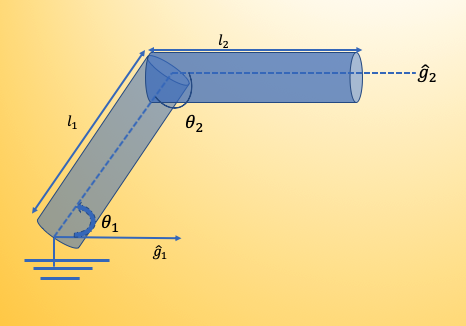
\includegraphics[width=.7\columnwidth]{figures/planar_manip.png}
	\caption{An illustration of the geometric configuration of the planar arm}
	\label{fig:planar_manip}
\end{figure}
%
\begin{subequations}
	\begin{align}
	\homo_1 = l_1 \cos \theta_1 + l_2 \nonumber \\
	%
	\homo_2 = l_1 \sin \theta_1 + l_2 \sin(\theta_1+\theta_2)
	\end{align}
\end{subequations}
% 
and whose first order time derivative yields,
%
\begin{subequations}
	\begin{align}
	\dot{\homo}_1 = -l_1 \dot{\theta}_1 \sin \theta_1  \nonumber \\
	%
	\dot{\homo}_2 = l_1 \dot{\theta}_1 \cos \theta_1 + l_2 (\dot{\theta}_1+\dot{\theta}_2) \cos(\theta_1+\theta_2).
	\end{align}
\end{subequations}
%
Vectorizing, we have
%
\begin{align}
	\left(\begin{array}{c}
		\dot{\homo}_1 \\
		%
		\dot{\homo}_2
	\end{array}\right) = \left(\begin{array}{cc}
	-l_1  \sin \theta_1 & 0 \\
	%
	 l_1  \cos \theta_1 + l_2  \cos(\theta_1+\theta_2) &  l_2 \dot{\theta}_2 \cos(\theta_1+\theta_2)
	\end{array}\right)
	%
	\left(\begin{array}{c}
	\dot{\theta}_1 \\
	%
	\dot{\theta}_2
	\end{array}\right)
\end{align}
% 
so that the velocity of the tip point of the 2R robot arm can be written as 
%
\begin{align}
	v_{tip} = J_1(\theta)\dot{\theta}_1 + J_2(\theta)\dot{\theta}_2.
\end{align}
%
We can always guarantee a tip point velocity as long as the columns of the manipulator Jacobian are not collinear. When collinearity occurs, the robot ends up in a \textit{singular configuration} and the Jacobian loses rank (more on this later on). Formally, we say a manipulator is in a singular configuration when the tip of the robot is unable to move arbitrarily in specific directions.

\subsection{The Manipulability Ellipsoid}
%
We now formally introduce the manipulability ellipsoid of the robot arm. When you start designing robot mechanisms, you would need to understand how arbitrarily changing the position and orientation of the end-effector at the tip of the robot arm is a function of the joint velocities and their positions. 
\begin{definition}
	The quantitative index that defines the set of all end-effector velocities that are realizable by joint velocities under a magnitude constraint (\eg a Euclidean norm  $<=1$) such that \textit{those end-effector velocities are \textbf{large and spherical} as much as possible} is the \textbf{manipulability measure} of the robot.
\end{definition}

The manipulability measures the performance of the arm's kinematics (motions) in order for us to optimize the size of the robot. To illustrate the intuitive mesaning of the manipulability measure, play with the cdf file located on the wolfram cloud at this \href{https://demonstrations.wolfram.com/ManipulabilityEllipsoidOfARobotArm/}{web address}. What happens, when you set all the angles of the robot to zero or $180^\circ$? Notice that the manipulability becomes $0$. Coincidentally, we find that this is a situation that occurs when the robot is at a singularity and the manipulability ellipsoid is at its lowest coverage within the manipulator workspace.

\begin{homework}
	Explain what happens when you adjust the parameters of the robot as follows 
	%
	\begin{itemize}
		\item Keep $\theta_1 = \theta_3 = 0$ and vary $\theta_2$. What do you notice about the size of the ellipsoid? How does it affect the mannipulability measure? 
		%
		\item Keep $\theta_2 = \theta_3 = 0$ and set $\theta_1$ at $\pi/2$. What happens to the shape of the ellipsoid? Report the manipulability measure.
		%
		\item Keep any  two the joints at $180^\circ$ and make the other joint $0^\circ$. What do you notice?
	\end{itemize}
\end{homework}

From the \href{http://scriptedonachip.com/downloads/Videos/manipulability.mp4}{video} of the ellipsoids, we notice that the closer the ellipsoids are in area to a circle, the more the freedom we obtain in being able to move the tip in arbitrary directions.  So we define the \textit{manipulability measure} as 
%
\begin{align}
	\sqrt{\dot{q}_1^2(t)+\dot{q}_2^2(t)+\ldots + \dot{q}_l^2(t)} \le 1
\end{align}
%
which is to say the the bound on the Euclidean norm of all joint angle velocities such that it is less than unity and we define the manipulability ellipsoid as 
%
\begin{align}
	\{ v(t) J^{-T} \cdot J^{-1} \cdot v(t) \le 1, v(t): Rank(J) \}
 \end{align}

\section{The Manipulator Jacobian}

Here, we are concerned with the magnitudes of the joint velocities when the  $\dot{\theta}_i = 1$ and all other joint velocities are $0$. This determines the twist, which we treated in \autoref{chap:rbm}. Particularly, we separate the treatments of the spatial manipulator Jacobian (\ie the the Jacobian where each column of $J$ is a screw axes in the base or a fixed spatial frame, $s$) and the body manipulator Jacobian (\ie the Jacobian where each column of $J$ is a screw axes in the the end-effector frame, $b$).

\subsection{Spatial Jacobian}
%
Consider the general Jacobian of \eqref{eq:jacob_gen}, suppose now that $g_{st} \rightarrow SE(3)$ is a forward kinematic map for the manipulator and the joints traverse a path $\theta(t) \in Q$, so that the end-effector follows a path $\homo_{st}(\theta(t)) \in SE(3)$. The instanteneous spatial velocity of the end-effector would be the set 
%
\begin{align}
	\hat{\eta}^s_{st} = \dot{\homo}_{st}(\theta) \homost^{-1}(\theta)
	\label{eq:spatial_jacob}
\end{align}
%
Applying the chain rule as before (\cf \eqref{eq:jacob_gen}), we have 
%
\begin{align}
	\hat{\eta}^s_{st}  = \sum_{i=1}^{n} \left(\dfrac{\partial \homo_{st}({\theta})}{\partial \theta_i} \dot{\theta}_i \right) \homost^{-1}(\theta) =  \sum_{i=1}^{n} \left( \dfrac{\partial \homo_{st}({\theta})}{\partial \theta_i} \homost^{-1}(\theta) \right) \dot{\theta}_i.
\end{align}
%
In twist coordinates, we write the above as 
%
\begin{align}
		\hat{\eta}^s_{st}  = J_{st}^s(\theta) \dot(\theta)
\end{align}
%
where
%
\[
	J_{st}^s = \left[\left(\dfrac{\partial \homo_{st}({\theta})}{\partial \theta_1} \homost^{-1}\right)^\vee 
							\ldots
						    \left(\dfrac{\partial \homo_{st}({\theta})}{\partial \theta_l} \homost^{-1}\right)^\vee 
							\right]
\]
%
and the $i'th$ joint twist transformed by $e^{\twistmap_1 \theta_1} \ldots e^{\twistmap_{i-1}\theta_{i-1}}$ from the $i'th$ joint in the reference configuration to the current configuration of the manipulator is
%
\[
	\left(\dfrac{\partial \homo_{st}({\theta})}{\partial \theta_1} \homost^{-1}\right)^\vee = \text{Ad}_{\left(e^{\twistmap_1 \theta_1}\ldots e^{\twistmap_{l-1} \theta_{l-1}}\right)}\twistmap_l :\equiv \twistcoord^\prime.
\]
%
It therefore follows that 
%
\begin{align}
	J_{st}^s(\theta) = \left[\twistcoord_1, \twistcoord_2^\prime  \ldots \twistcoord^\prime_l \right]
\end{align}
%
We thus see that the \textit{i'th column of the Jacobian corresponds to the i'th joint twist, transformed to the current manipulator configuration.}

\subsection{The Body Jacobian}
%
In body coordinates, we rewrite \eqref{eq:spatial_jacob} as 
%
\begin{align}
\hat{\eta}^b_{st} = J^b_{st}(\theta)\dot{\theta}
\label{eq:body_jacob}
\end{align}
%
so that 
%
\begin{subequations}
	\begin{align}
	J_{st}^b(\theta) =  \left[\twistcoord_1^\star, \twistcoord_2^\star  \ldots \twistcoord^\star_{l-1} \twistcoord^\star_{l} \right] \\
	%
	\twistcoord_i^\star = \text{Ad}^{-1}_{\left(e^{\twistmap_1 \theta_1}\ldots e^{\twistmap_{l} \theta_{l}}\homost(0)\right)}\twistmap_i
	\end{align}
\end{subequations}
%
where the $\homost(0)$ term allows us the freedom to choose the base frame in order to simplify our calculations (\eg choose $\homost(0) = I$.

Before we close this section, we note the following relations between the two Jacobians:
%
\begin{align}
	J_{st}^s(\theta) = Ad_{\homost(\theta}J_{st}^b(\theta).
\end{align}
%
These spatial and body manipulator Jacobians are useful in finding the instanteneous velocity of the tip point in the end-effector frame. Suppose we let $q^b$ be this tip point in body coordinates, we can find the velocity $v^b$ in the tool frame (body coordinates) as 
%
\begin{align}
	v^b_q = \hat{\eta}_{st}^b q^b = \left(J_{st}^b(\theta) \dot{\theta}\right)^\wedge q^b.
\end{align}
%
The logic above applies in spatial coordinates (\ie the base frame), whereupon we have
%
\begin{align}
v^s_q = \hat{\eta}_{st}^s q^s = \left(J_{st}^s(\theta) \dot{\theta}\right)^\wedge q^s
\end{align}

Notice from \eqref{eq:spatial_jacob} that 
%
\begin{align}
	\dot{\theta}(t) = \left(J_{st}^s(\theta)^{-1} \eta_{st}^s (t) \right)
\end{align}
%
implying that we do not need the inverse kinematics of the manipulator of the robot if we want to move an arm from one end-effector pose to another since we know the relationship between the joint velocities and the end-effector velocity.

\begin{homework}
	Explain how you would go about implementing the last part of the above statement for the planar robot arm of \autoref{fig:planar_manip}.
\end{homework}

\section{Inverse kinematics}
%
We formally define the inverse kinematics problem as follows: given a desired configuration for the end-effector, $\homo_d$, find the joint angles necessary for achieving that configuration. Mathematically, we can think of this as being given a forward kinematic map $\homost: Q \rightarrow SE(3)$, and $\homo_d$, find the desired joint angles by solving 
%
\begin{align}
	\homost(\theta) = \homo_d
\end{align}
%
for some $\theta \in Q$. It is noteworthy to here point out that the IK problem mat have multiple solutions,, a unique solution or no solution at all. It is typical to use numerical optimization approaches to solve these problems in practice. In ROS, there are different IK libraries that are available such as the ones from \textsc{KDL} or 

\begin{example}
	Consider the two-link planar arm of \autoref{fig:ik_ex}. We know the forward kinematics to be 
	%
	\begin{align}
		content...
	\end{align}
\end{example}

\begin{figure}[tb!]
	\centering
	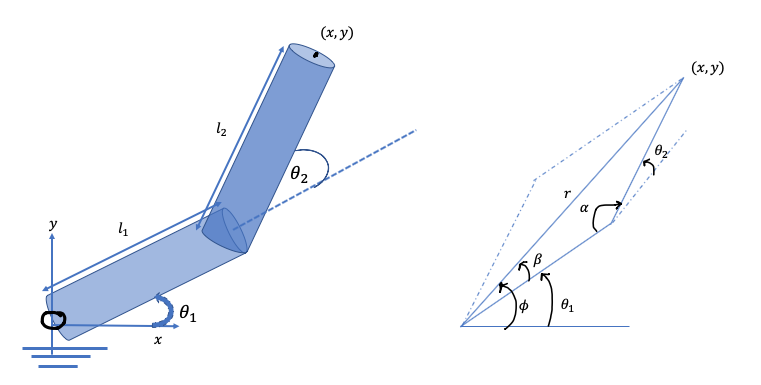
\includegraphics[width=.8\columnwidth]{figures/ik_ex.png}
	\caption{Inverse Kinematics of a two-link planar manipulator}
	\label{fig:ik_ex}
\end{figure}